\section{Resonance resolution}
\label{sec:res}
% 
The final component of the mass resolution is due to the uncertainties
on the parameters of the $J/\psi$ resonance. This component is
relatively small ($0.6 \mevc$ for the $\chicone$ decay given the
numbers in Table \ref{tab:rescontrib}) due to the mass constraint applied in the kinematic
fit. Since the uncertainties from the decay tree fit for these
parameters were not stored on the ntuple a different approach was
used. The adopted procedure was to fit the difference between the true and reconstructed values of the
$J/\psi$ slopes and momentum in slices and parameterize the
result. For the slopes the form give in Equation \ref{eq:sloperes}, with $A_{res} = 2.9 \times 10^{-5}$ and $B_{ms} =
7.5 \mevc$, is found to fit well (Fig. \ref{fig:resty}).  
%
\begin{figure}[htb!]
%\vspace{-5mm}
\begin{center}
\resizebox{3.5in}{!}{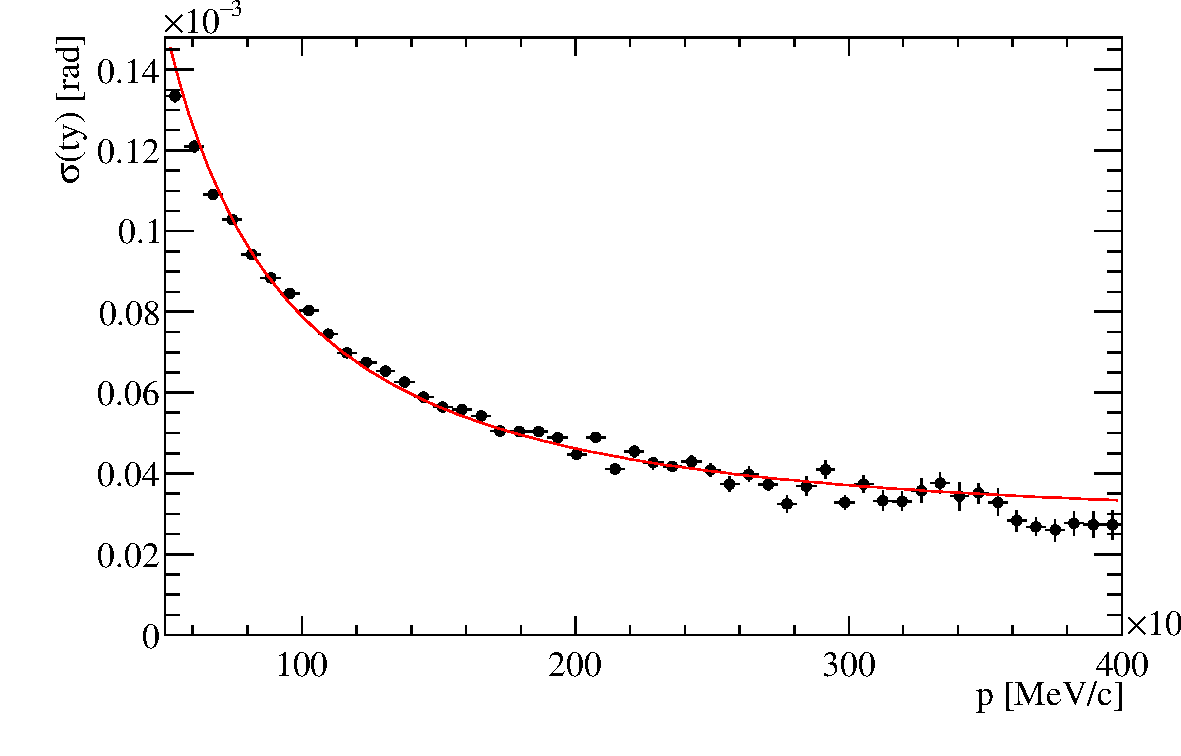
\includegraphics{figs/resty.pdf}}
%\vspace{-5mm}
\caption{\small Resolution on the $J/\psi$ slope in $ty$. A fit to the
  form discussed in the text is superimposed.} 
\label{fig:resty}
\end{center}
\end{figure}

For the uncertainty from the $J/\psi$ momentum no aesthetically pleasing
parameterization is found (Fig. \ref{fig:resp}) and the distribution is
modelled with a $4^{th}$ order polynomial.

\begin{figure}[htb!]
%\vspace{-5mm}
\begin{center}
\resizebox{3.5in}{!}{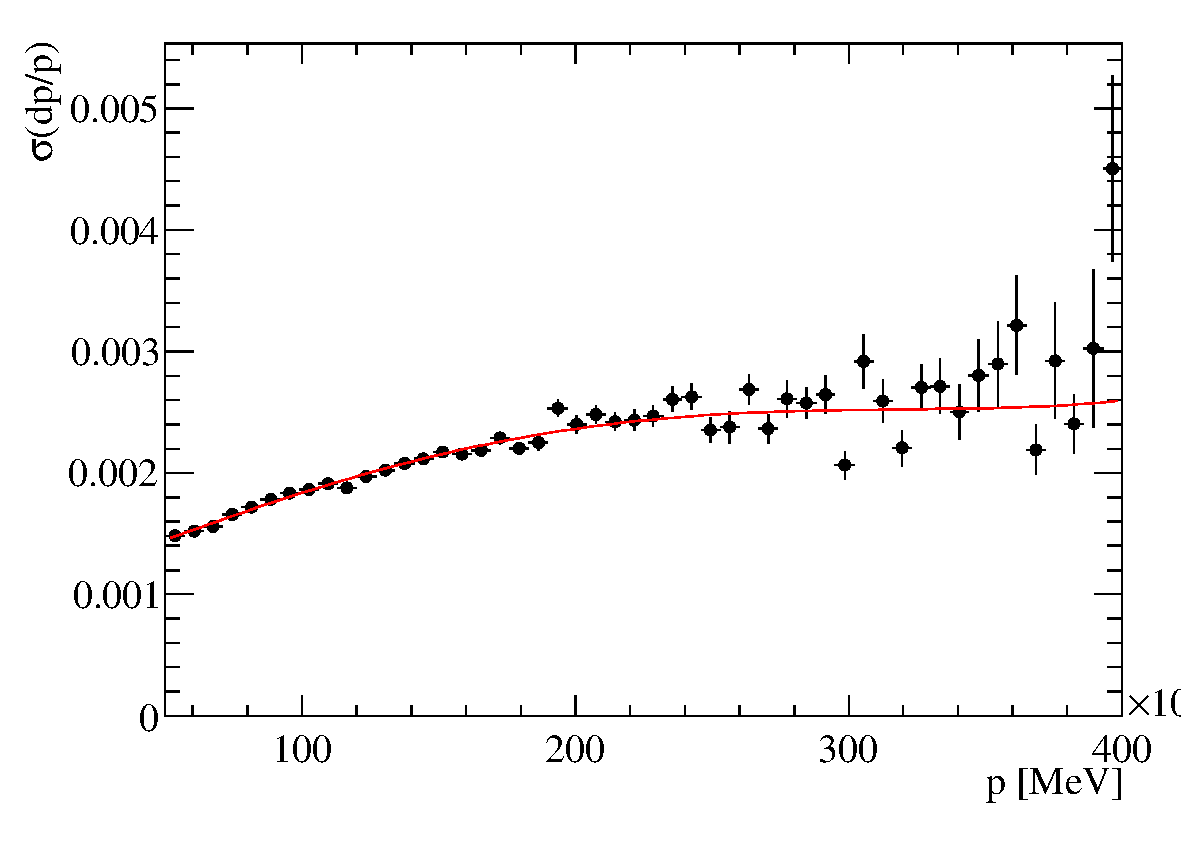
\includegraphics{figs/resp.pdf}}
%\vspace{-5mm}
\caption{\small Resolution on the $J/\psi$ momentum as function of
  momentum. A fit to a fourth order polynomial is superimposed. The
  polynomial parameters (with $p$ in $\mevc$) are $1 \times 10^{-3}, 7
\times 10^{-9}, 1 \times 10^{-14}, -1.2 \times 10^{-19}, 1.7 \times 10^{-25} $. }
\label{fig:resp}
\end{center}
\end{figure}
